\documentclass[10pt]{article}
\usepackage[margin=0.7in]{geometry}
\usepackage{graphicx}
\usepackage{booktabs}
\usepackage{amsmath}
\begin{document}
\begin{center}
{\Large Fixed-base N53 S3 root-batch result}\par
Nine verified single-target pairs, 2026-10-12
\end{center}
\noindent\textbf{Question.} Does batching inversions in the second S3
root call reduce charged rank and target work under the exact fixed K220
base and rank stream? Curve EC1N53Ce0hb097de99be9a, subgroup
order 21,044,858,204,113. The frozen source, public inputs and binary
hashes are in \texttt{FROZEN.json}; raw runs in \texttt{runs/};
native exact/replay verdict in \texttt{ANALYSIS.json} and aggregate in
\texttt{RESULT\_DATA.json}.

\smallskip
\noindent\textbf{Verified result.} All 27 valid fresh processes
completed; all nine IC pairs reached rank 220/220 with 220 independent
relations each. Native replay checked each relation, factor log and
target scalar. The control and batch arms retain the same base, selected
rank trace, root table, consumed roots and target witness. Exact and
inversion gates passed.

\begin{center}
\begin{tabular}{lrrl}
\toprule
Same-Q ratio, in-process ms & Median & 95\% block interval & Scope\\
\midrule
Control/strong rho, cold & 78.146 & [44.220, 92.602] & L0 diagnostic\\
Batch/strong rho, cold & 52.586 & [33.179, 64.668] & L0 diagnostic\\
Batch/control, cold & 0.738 & [0.714, 0.750] & L0 diagnostic\\
Control/strong rho, online & 0.490 & [0.168, 0.763] & L0 diagnostic\\
Batch/strong rho, online & 0.378 & [0.103, 0.442] & L0 diagnostic\\
Batch/control, online & 0.612 & [0.569, 0.903] & L0 diagnostic\\
\bottomrule
\end{tabular}
\end{center}
\noindent The candidate/control descriptive gates were cold
\(\leq 0.90\) and online \(\leq 1.10\), both met. Bootstrap intervals
come from 10,000 deterministic resamples of three public-target blocks;
each block retains its three rank seeds. The host was a shared Apple M4
Pro, macOS 26.6, with no core isolation. Rho uses the same Q, strong
rung 3, 32 lanes and DP4.

\smallskip
\noindent\textbf{Charged root primitives, nine IC cells.}
Control versus batch: 80,790,012 versus 763,167 inversions
(ratio 0.009446); 1,211,850,180 versus 902,063,394 field
multiplication calls (0.744369); 242,370,036 versus 39,684,684
squaring calls (0.163736). Extra prefetched roots are charged.
This is engineering with unchanged relations, not a measured generic
exponent change. The complete-operation unit
\(S=\mathrm{GAE}/\sqrt{r}\) and ratio to its
\(\sqrt{\pi/(2\cdot106)}\) floor remain uncalibrated.
The cold IC/rho ratios are above 1 in every pair.
Host-isolated timing and second-host replay remain open.

\smallskip
\noindent\textbf{Custody and validation.} The executable source commit
was \texttt{00a8da2d}; public inputs and binary hashes were pushed in
\texttt{576f7087b} before timing. A sandboxed \texttt{time -l}
measurement-wrapper attempt returned incomplete statuses and is preserved
separately; the valid run used the same source, inputs and schedule outside
that sandbox. Final validation: 4,000 release library tests, 22 release
example tests and four targeted scoreboard/site tests passed. The full
site suite has one unrelated baseline error: the preverified cover report
names a registry digest that differs from the unchanged registry on
\texttt{origin/main}. The canonical scoreboard and timeline carry only
L0 diagnostic points. A ledger promotion remains pending common-\(S\)
calibration and an admitted isolated reference.

\clearpage
\begin{center}
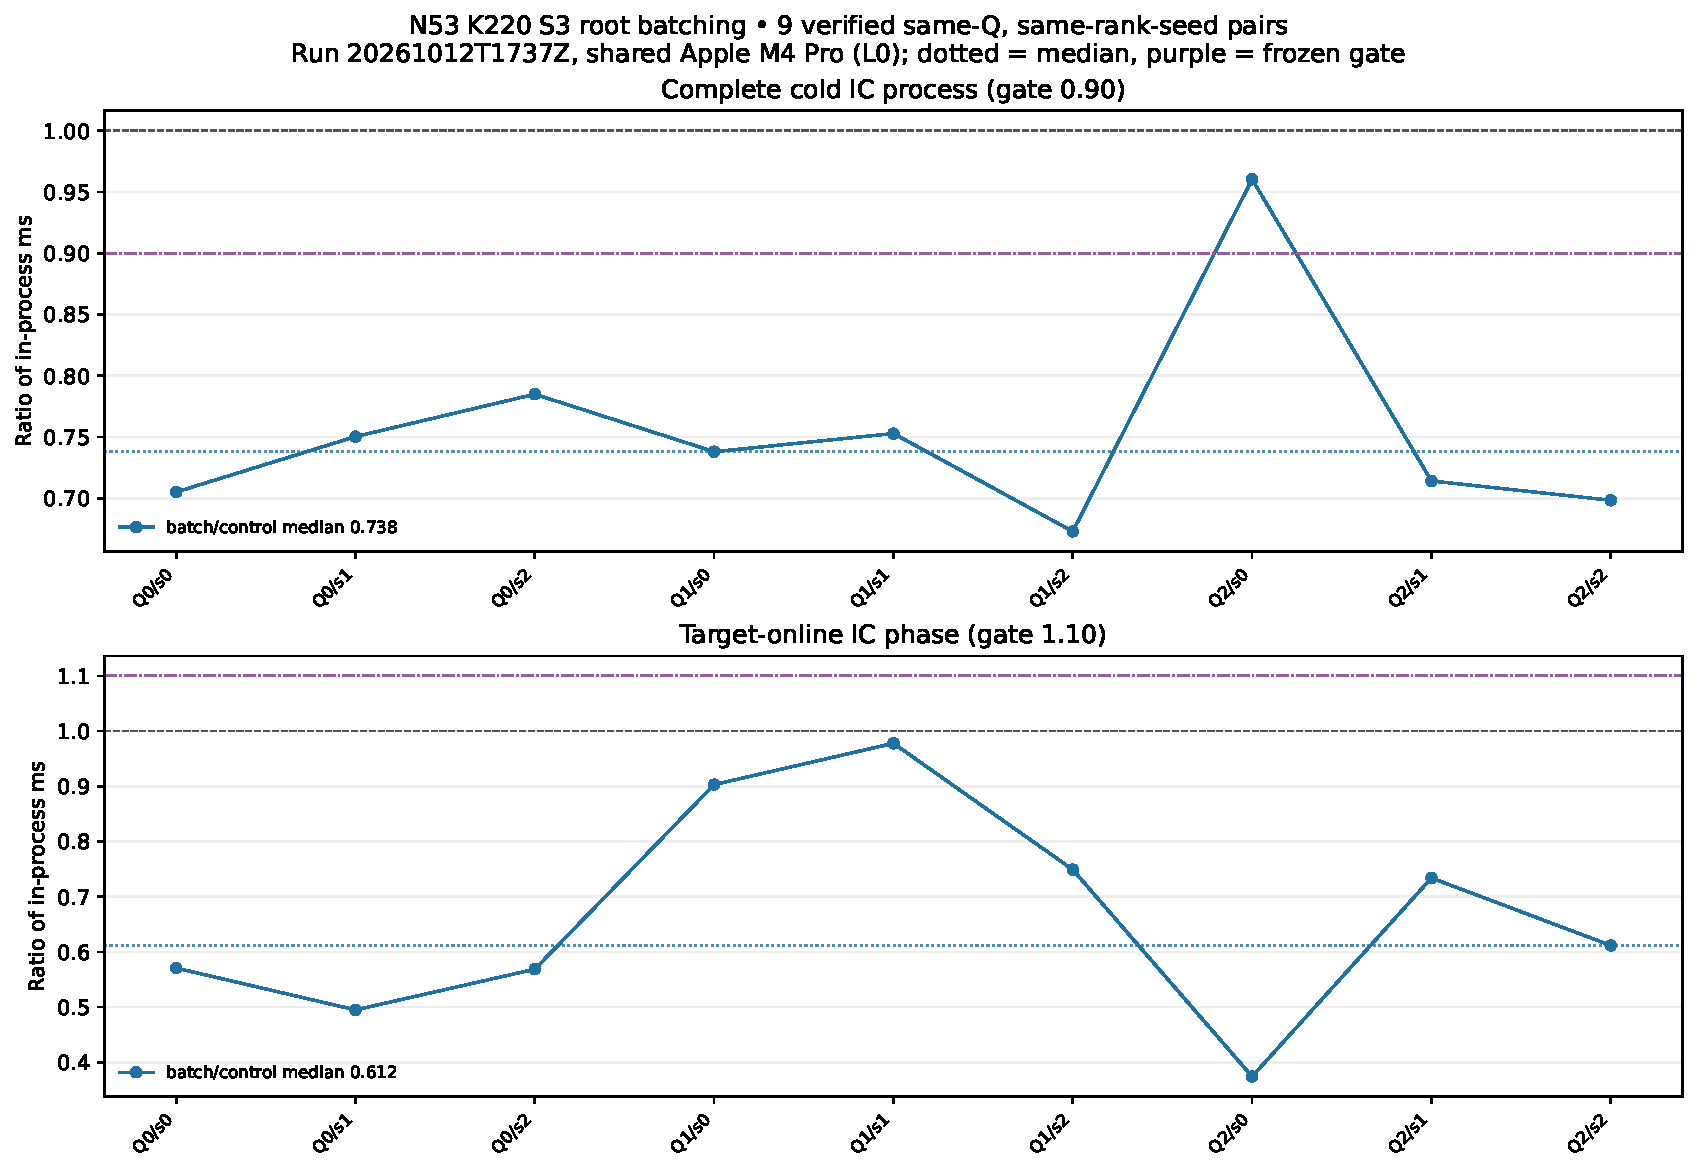
\includegraphics[width=\linewidth]{reports/run-20261012T1737Z/paired_ratios.pdf}
\end{center}
\clearpage
\begin{center}
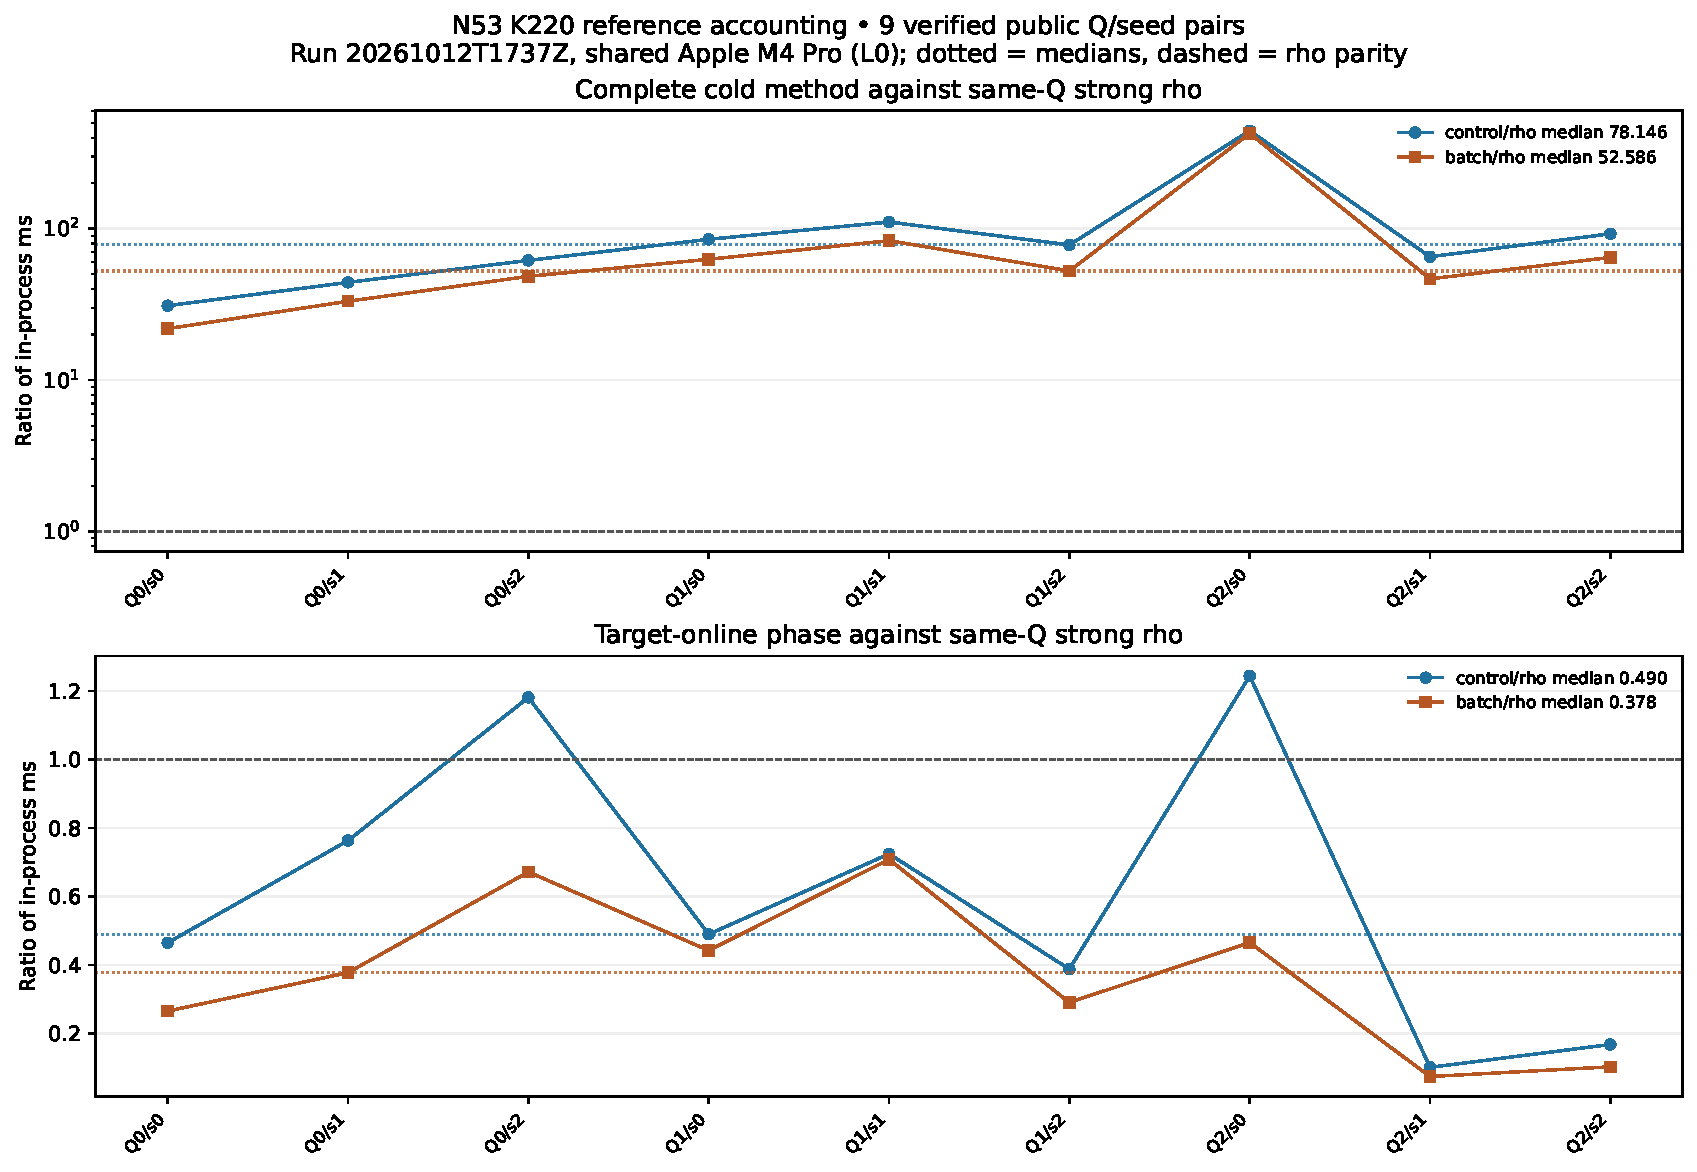
\includegraphics[width=\linewidth]{reports/run-20261012T1737Z/rho_reference.pdf}
\end{center}
\end{document}
